\documentclass{article}
\usepackage{graphicx} % Required for inserting images
\usepackage{hyperref}
\usepackage[
    backend = biber,
    style = abnt,
    ]{biblatex}
\addbibresource{bibliografia.bib}
\usepackage[shortlabels]{enumitem}
\usepackage[brazilian]{babel}

\title{%
  Direito Internacional Público \\
  \Large Notas de Aula 4\\
  \Large Fontes do DIP/Tratados p. 2\\
  }
\author{Luccas Gissoni}
\date{17 de setembro de 2024}

\begin{document}

\maketitle


\tableofcontents

\section{Classificação}

Os tratos podem ser classificados em função:

\subsection{Do número de Estados-parte:}

\begin{enumerate}[(a)]
    \item \textbf{bilaterais:} celebrados entre duas partes;
    \item \textbf{plurilaterais:} celebrados por mais de duas partes;
    \item \textbf{multilaterais:}  celebrados por mais de duas partes, no interior de uma organização internacional;
\end{enumerate}

\subsection{Da generalidade de suas disposições:}

\begin{enumerate}[(a)]
    \item \textbf{convenções gerais:} ``também conhecidas como \textbf{convenções-quadro ou guarda-chuva}: as quais estabelecem normas e princípios gerais que serão detalhados posteriormente por meio de tratados internacionais específicos, por meio de protocolos adicionais ou mesmo por meio de legislação interna; geralmente são utilizados em situações de difícil consenso político entre as partes (meio ambiente, saúde, minorias, entre outros)" \cite[p.~153]{accioly_manual_2023};
    \item \textbf{convenções específicas:} ``as quais adotam de forma detalhada normas jurídicas específicas sobre o tema regulado, com o objetivo de esgotar em seu próprio instrumento tal regulação" \cite[p.~153]{accioly_manual_2023};
\end{enumerate}

\subsection{Da natureza jurídica:}

Refere-se à natureza jurídica das normas consolidadas no tratado. Aqui, há duas subclassificações possíveis, em função:

\subsubsection{Da imperatividade da norma:}

\begin{enumerate}[(a)]
    \item \textbf{tratado de direito dispositivo:} normas podem ser derrogadas por meio de tratado posterior;
    \item \textbf{tratado de direito cogente (\textit{jus cogens}):} as \textbf{normas imperativas de direito internacional geral} sobre matérias cuja natureza não comportaria derrogação mesmo diante de acordo formalizado em sentido diverso:
\end{enumerate}

\begin{quote}
\begin{center}
    Artigo 53

Tratado em Conflito com uma Norma Imperativa de Direito

Internacional Geral (\underline{jus cogens})
\end{center} 

É nulo um tratado que, no momento de sua conclusão, conflite com uma norma imperativa de Direito Internacional geral. Para os fins da presente Convenção, uma norma imperativa de Direito Internacional geral é uma norma aceita e reconhecida pela comunidade internacional dos Estados como um todo, como norma da qual nenhuma derrogação é permitida e que só pode ser modificada por norma ulterior de Direito Internacional geral da mesma natureza \cite{brasil_decreto_2009}.
\end{quote}

\subsubsection{Do tipo de interesse juridicamente regulado:}

\begin{enumerate}[(a)]
    \item \textbf{tratados-contratos:} regulam interesses recíprocos dos Estados, geralmente de caráter bilateral (interesse bilateral barganhado);
    \item \textbf{tratados-leis ou tratados-normativos:} fixam normas de direito internacional geral (interesse geral).
\end{enumerate}

\section{Condição de validade do tratado}

Para que o tratado seja considerado válido, é necessário que:

\begin{itemize}
    \item as partes (Estados ou organizações internacionais) tenham capacidade para celebrá-los;
    \item os agentes estejam habilitados;
    \item haja consentimento mútuo;
    \item o seu objeto seja lícito e possível.
\end{itemize}

\subsection{Capacidade das partes contratantes}

\begin{quote}
    \begin{center}
         Artigo 6

        Capacidade dos Estados para Concluir Tratados
    \end{center}
Todo Estado tem capacidade para concluir tratados \cite{brasil_decreto_2009}.
    
\end{quote}

Tornou-se obsoleta a doutrina de que apenas os Estados têm capacidade de celebrar tratados. Com a Carta das Nações Unidas, passou-se a aceitar, de início timidamente, a capacidade das organizações internacionais. Atualmente, a questão foi pacificada, com destaque para a Convenção de Viena sobre o Direito dos Tratados entre Estados e Organizações Internacionais ou entre Organizações Internacionais, de 1986, que trata especificamente da questão.

\subsection{Habilitação dos agentes}

\begin{quote}
    Para a adoção ou autenticação do texto de um tratado, ou para expressar o consentimento do estado em obrigar-se a suas disposições, é necessário que os representantes demonstrem deter a autorização para tanto mediante a apresentação dos plenos poderes. Este documento indica que determinada pessoa é reconhecida pelo estado que ela representa como detendo plenos poderes para negociar e assinar um tratado internacional especificamente indicado em tal documento \cite[p.~155]{accioly_manual_2023}.
\end{quote}

\begin{quote}
    \begin{center}
         Artigo 7

        Plenos Poderes 
    \end{center}
    
    \begin{enumerate}
        \item Uma pessoa é considerada representante de um Estado para a adoção ou autenticação do texto de um tratado ou para expressar o consentimento do Estado em obrigar-se por um tratado se: 
    
            \begin{enumerate}[a)]
                \item apresentar plenos poderes apropriados; ou 
                \item a prática dos Estados interessados ou outras circunstâncias indicarem que a intenção do Estado era considerar essa pessoa seu representante para esses fins e dispensar os plenos poderes. 
            \end{enumerate}

        \item Em virtude de suas funções e independentemente da apresentação de plenos poderes, são considerados representantes do seu Estado: 
    
            \begin{enumerate}[a)]
                \item os Chefes de Estado, os Chefes de Governo e os Ministros das Relações Exteriores, para a realização de todos os atos relativos à conclusão de um tratado; 
                \item os Chefes de missão diplomática, para a adoção do texto de um tratado entre o Estado acreditante e o Estado junto ao qual estão acreditados; 
                \item os representantes acreditados pelos Estados perante uma conferência ou organização internacional ou um de seus órgãos, para a adoção do texto de um tratado em tal conferência, organização ou órgão.
            \end{enumerate}
    
    \end{enumerate}
    \cite{brasil_decreto_2009}

\end{quote}

\begin{quote}
    No que se refere às organizações internacionais, o órgão habilitado a negociar tratados internacionais está usualmente definido no texto de seu tratado constitutivo. Cada organização internacional possui um tratado internacional que a constitui e, por esse motivo, cada uma delas estabelece um procedimento próprio para se vincular juridicamente a um tratado internacional \cite[p.~155-156]{accioly_manual_2023}.
\end{quote}

\subsection{Consentimento mútuo}

O tratado é acordo de vontades, efetivando-se pelo consentimento:

\begin{quote}

    \begin{center}
         Artigo 9

        Adoção do Texto 
    \end{center}

    \begin{enumerate}
        \item A adoção do texto do tratado efetua-se pelo consentimento de todos os Estados que participam da sua elaboração, exceto quando se aplica o disposto no parágrafo 2.
        \item A adoção do texto de um tratado numa conferência internacional efetua-se pela maioria de dois terços dos Estados presentes e votantes, salvo se esses Estados, pela mesma maioria, decidirem aplicar uma regra diversa.
    \end{enumerate}

    \cite{brasil_decreto_2009}
\end{quote}

\subsection{Objeto lícito e possível}

Assim como no direito interno, só se pode visar coisa materialmente possível e permitida peo direito e pela moral. A doutrina menciona o Acordo de Munique, de 1938, em que o Reino Unido, a França, a Alemanha e a Itália negociaram a entrega dos Sudetos tchecos a Berlim sem a participação da Checoslováquia (Figuras \ref{fig:acordo_munique} e \ref{fig:particao_checoslovaquia}).

\begin{figure}
    \centering
    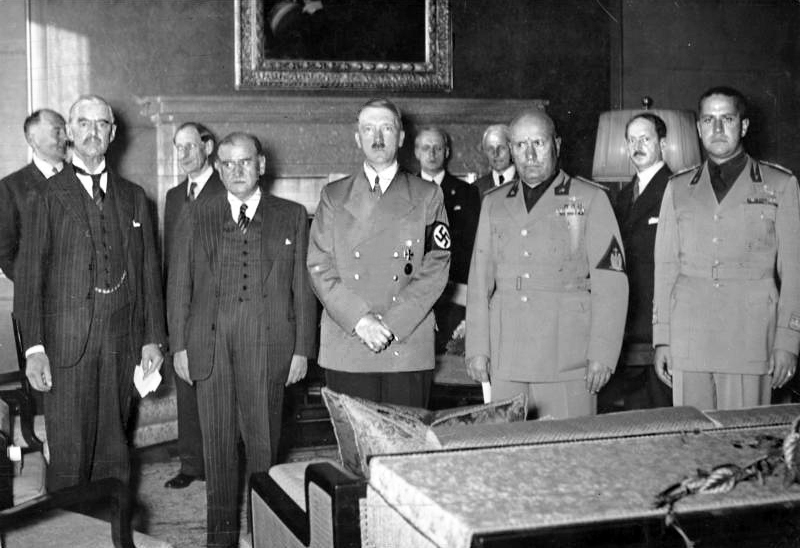
\includegraphics[width=0.85\linewidth]{acordo_munique.jpg}
    \caption{Da esquerda para direita: Chamberlain, Daladier, Hitler, Mussolini e Ciano após a assinatura do Acordo de Munique. Por Bundesarchiv, Bild 183-R69173 / CC-BY-SA 3.0}
    \label{fig:acordo_munique}
\end{figure}

\begin{figure}
    \centering
    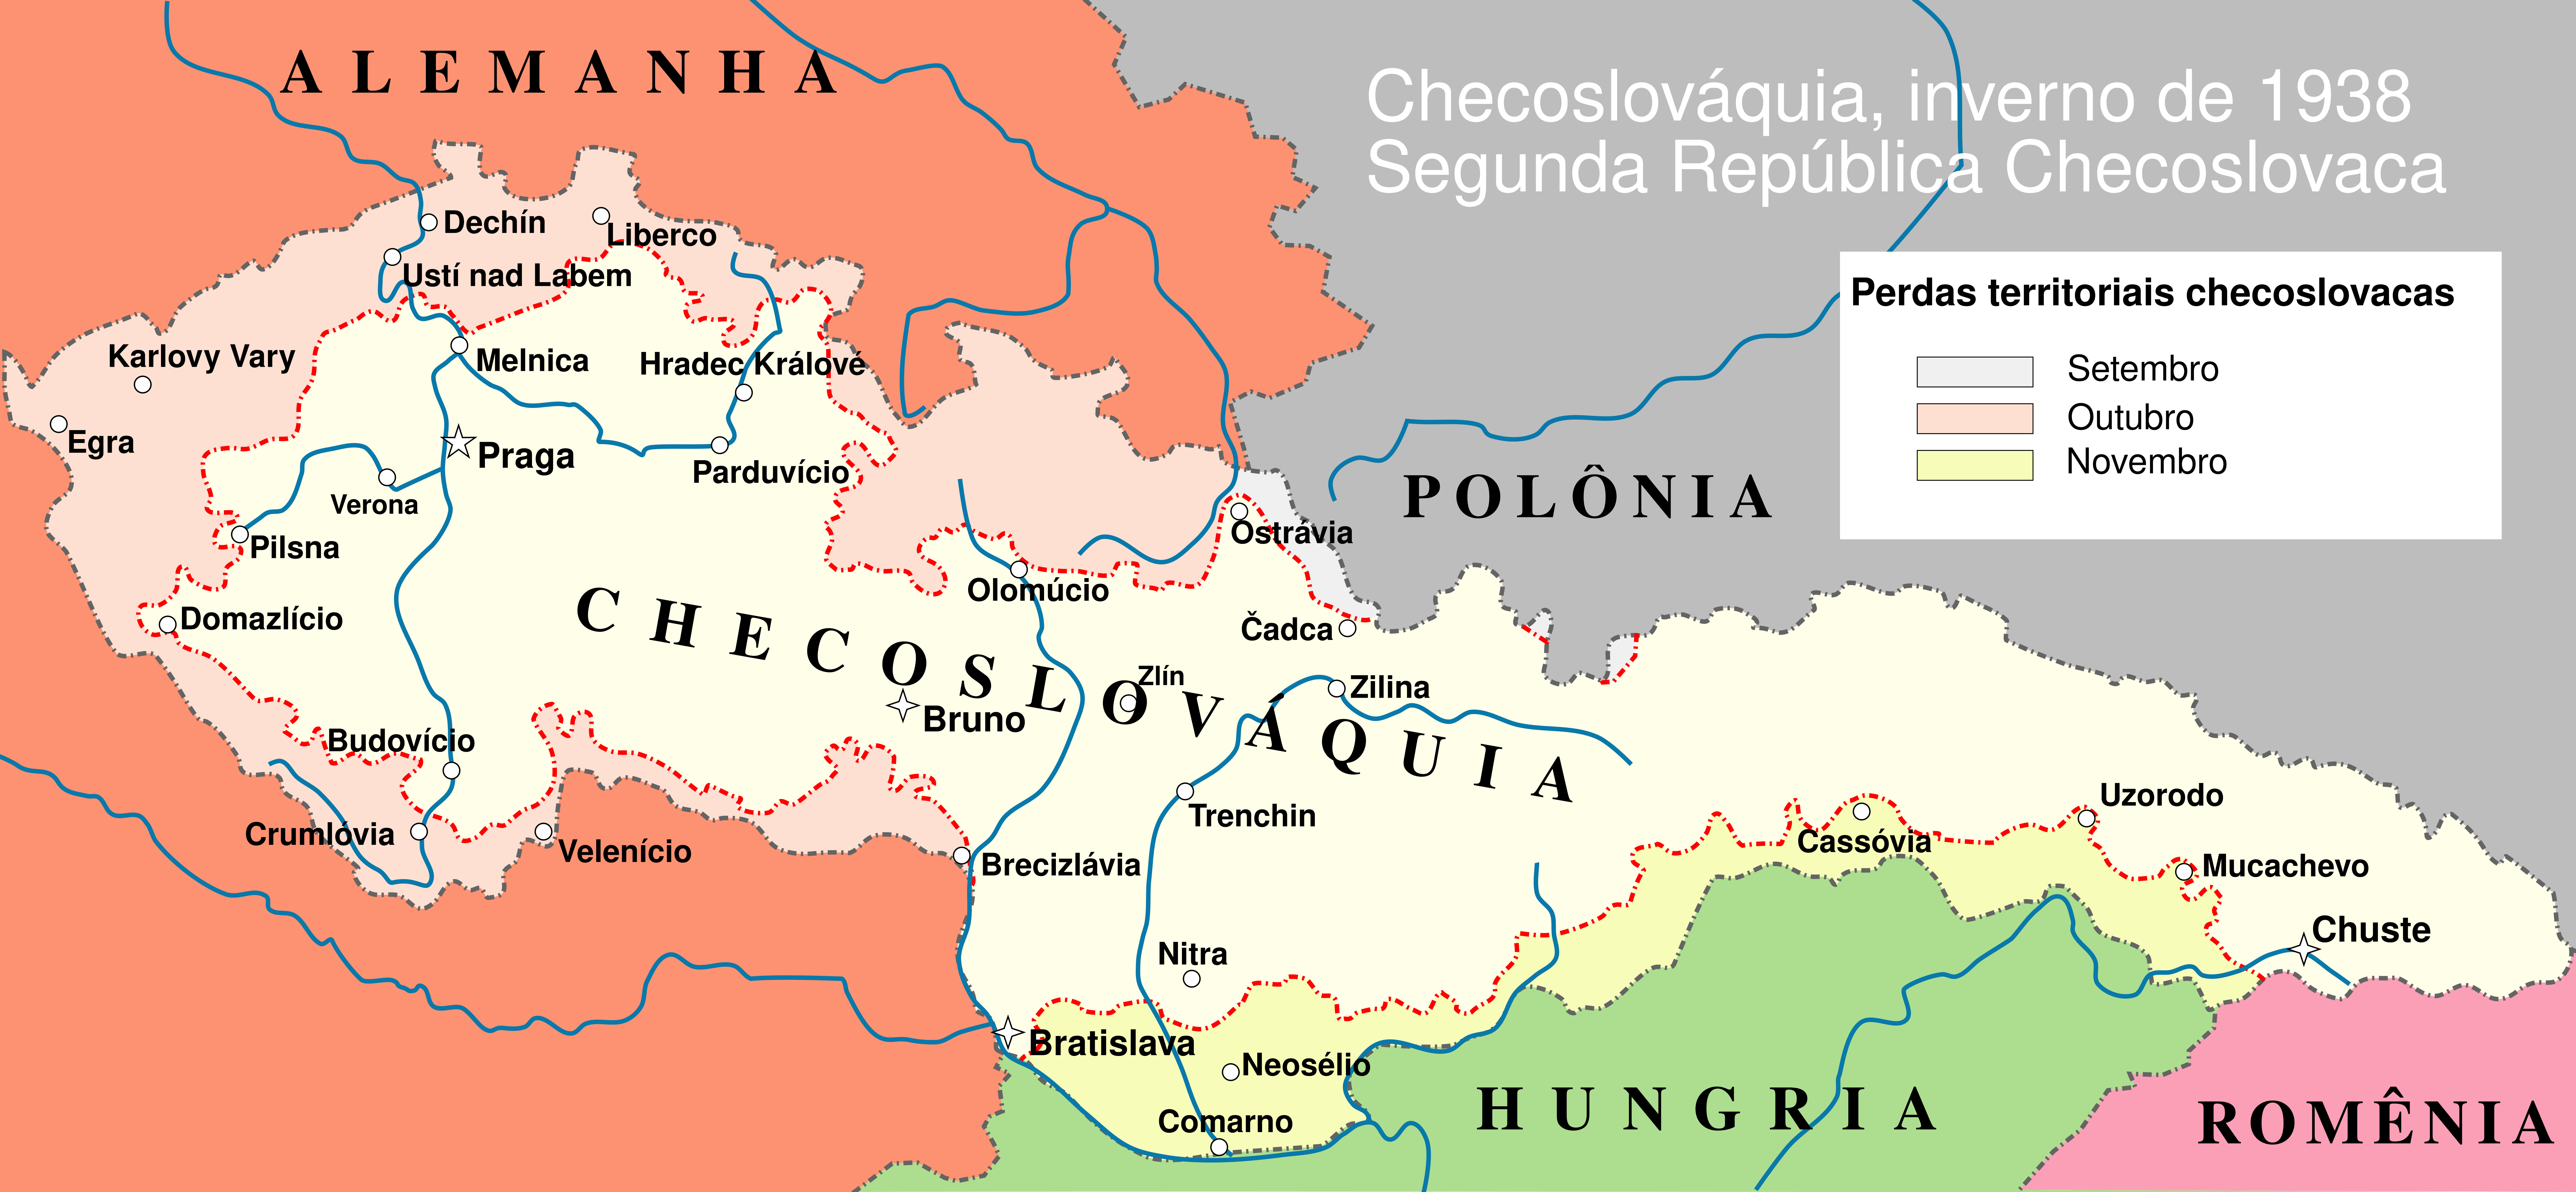
\includegraphics[width=0.85\linewidth]{particao_checoslovaquia.jpg}
    \caption{Partição da Checoslováquia (1938)}
    \label{fig:particao_checoslovaquia}
\end{figure}

\section{Efeitos em relação a terceiros}

\begin{quote}
    \begin{center}
         SEÇÃO 4

        Tratados e Terceiros Estados 
        
        Artigo 34
        
        Regra Geral com Relação a Terceiros Estados
    \end{center}
    Um tratado não cria obrigações nem direitos para um terceiro Estado sem o seu consentimento.
    \cite{brasil_decreto_2009}
\end{quote}

Decorre da soberania dos Estados e da autonomia da vontade o princípio de que ``um tratado só faz lei entre os estados que nele são parte”. Trata-se da regra \textit{res inter alios acta aliis neque nocere neque prodesse potest} (coisa pactuada não pode causar danos nem vantagens a terceiros).

\begin{quote}
    Todavia, se um tratado não pode ser fonte nem de direitos nem de obrigações para terceiros, não se deve deixar de notar que os tratados podem produzir consequências a estados terceiros:
    \begin{enumerate} [1º)]
        \item se \textbf{nocivas}, o estado lesado tem o direito de protestar e de procurar assegurar os seus direitos, bem como o de pedir reparações; se, entretanto, o tratado não viola direitos de estado não contratante e é apenas prejudicial a seus interesses, ou lhe causa dano legal, ou antes damnum sine injuria, o estado lesado poderá reclamar diplomaticamente contra o fato, mas contra o mesmo não terá recurso jurídico;
        \item caso sejam as consequências \textbf{favoráveis} para estados que do tratado não participem, ou que os contratantes, por manifestação de vontade expressa, concedam direito ou privilégio a terceiros (arts. 36 a 38). A bem dizer, essa é a única hipótese de exceção ao princípio de que o tratado só produz efeitos entre as partes contratantes.
    \end{enumerate}
    \cite[p.~157]{accioly_manual_2023}
\end{quote}

\section{Assinatura, ratificação e reservas}

\begin{quote}
    \begin{center}
         Artigo 11

        Meios de Manifestar Consentimento em Obrigar-se por um Tratado
    \end{center}
    O consentimento de um Estado em obrigar-se por um tratado pode manifestar-se pela assinatura, troca dos instrumentos constitutivos do tratado, ratificação, aceitação, aprovação ou adesão, ou por quaisquer outros meios, se assim acordado.
    \cite{brasil_decreto_2009}
\end{quote}

\subsection{Assinatura}

\begin{quote}
    Em regra, a simples assinatura não vincula juridicamente um estado ao tratado internacional. A assinatura por si só possui um sentido muito mais político do que jurídico: apresenta o estado simbolicamente como um ator que concorda com a importância do que foi discutido – ainda que a ele não se vincule no futuro. E ainda que não tenha participado da negociação. A assinatura funciona assim mais como um atestado de que o texto final corresponde fielmente ao que foi discutido pelos estados durante o período de negociação – e, por isso mesmo, ela não tem o papel de vincular juridicamente o estado \cite[p.~159]{accioly_manual_2023}.
\end{quote}

\subsection{Ratificação}

\begin{quote}
    (E)m regra,\footnote{``Todavia, quando a assinatura for considerada pelo próprio tratado como definitiva, isso significa que as partes compreendem ser desnecessária a ratificação. A dispensa da ratificação ocorre quando o próprio tratado assim dispuser; nos acordos celebrados para cumprimento ou interpretação de tratado devidamente ratificado; nos acordos sobre assuntos puramente administrativos, que preveem eventuais modificações, como no caso de acordos de transporte aéreo; nos modus vivendi, que têm por finalidade deixar as coisas no estado em que se acham ou estabelecer simples bases para negociações futuras. Nos tratados sobre o meio ambiente tem surgido a prática de assinar tratados-base (convenções-quadro), que traçam as grandes linhas e que devem ser completados por protocolos ou pela modificação de anexos em que a ratificação pode ser dispensada. Nestas situações, basta a assinatura para o estado se vincular juridicamente ao tratado" \cite[p.~159]{accioly_manual_2023}.} a vinculação jurídica de um estado a um tratado apenas ocorre por meio da ratificação. Esta consiste em um ato administrativo mediante o qual o chefe de estado confirma tratado firmado em seu nome ou em nome do estado, declarando se submeter ao regime jurídico ali disposto \cite[p.~159]{accioly_manual_2023}.
\end{quote}

Normalmente, a ratificação (pelo chefe do Poder Executivo) fica condicionada à \textbf{aprovação} do tratado pelo Poder Legislativo. No caso da Constituição Federal de 1988:

\begin{quote}
    Art. 84. Compete privativamente ao Presidente da República:\\
    (...)\\
    VIII - celebrar tratados, convenções e atos internacionais, sujeitos a referendo do Congresso Nacional;
\end{quote}

E ainda:

\begin{quote}
    Art. 49. É da competência exclusiva do Congresso Nacional:\\
    I - resolver definitivamente sobre tratados, acordos ou atos internacionais que acarretem encargos ou compromissos gravosos ao patrimônio nacional; 
\end{quote}

O direito internacional nção prescreve forma necessária à ratificação. Normalmente, contudo, ela ocorre por meio do depósito da \textbf{carta de ratificação} junto ao organismo multilateral pertinente, ou pela sua troca por outro documento idêntico, produzido pela outra parte contratante. Tal documento, assinado pelo Chefe de Estado e Ministro das Relações Exteriores, contém a promessa de que o tratado será cumprido inviolavelmente, mas é a troca em si, que expressa o consentimento, o que torna o tratado perfeito e acabado.

\subsection{Reservas}

\begin{quote}
    Quando da assinatura ou da vinculação jurídica a um tratado (ratificação ou adesão), um estado por apresentar reservas ao documento. A reserva é um ato unilateral de estado, por meio do qual ele afasta ou modifica a aplicação de uma disposição de um tratado em relação a ele mesmo. Em outras palavras, ele se reserva o direito a não se vincular a determinado trecho do tratado.\\

    O problema das reservas a tratados bi ou multilaterais tem sido um dos mais complexos em direito internacional. Durante muito tempo a doutrina era no sentido de que um tratado só podia ser ratificado tal qual foi assinado: ou deveria ser aprovado integralmente, ou rejeitado (single undertaking), pois as disposições apenas fazem sentido como um todo integrado e devidamente negociado como um conjunto.\\
    
    O problema das reservas a tratados multilaterais agravou-se com as Nações Unidas e o aumento dos estados-membros da comunidade internacional, e constatou-se que a antiga regra tornara-se inexequível. Em 1951, a CIJ foi chamada a opinar sobre as reservas formuladas à Convenção sobre genocídio, e em seu parecer manifestou-se no sentido de que um estado, parte numa convenção, tem o direito de objetar às reservas que considere incompatíveis com o objeto e a finalidade da citada convenção e considerar o estado que formulou as reservas como não vinculado à Convenção\cite[p.~162]{accioly_manual_2023}.
\end{quote}

\begin{quote}
    \begin{center}
         Artigo 19

        Formulação de Reservas 
    \end{center}    
    Um Estado pode, ao assinar, ratificar, aceitar ou aprovar um tratado, ou a ele aderir, formular uma reserva, a não ser que:
    \begin{enumerate}[a)]
        \item a reserva seja proibida pelo tratado; 
        \item o tratado disponha que só possam ser formuladas determinadas reservas, entre as quais não figure a reserva em questão; ou
        \item nos casos não previstos nas alíneas a e b, a reserva seja incompatível com o objeto e a finalidade do tratado.
    \end{enumerate}\cite{brasil_decreto_2009}
\end{quote}

\section{Interpretação}

Como regra geral, o tratado deve ser interpretado segundo o princípio da boa-fé.

\begin{quote}
    \begin{center}
         Artigo 31

        Regra Geral de Interpretação
    \end{center}    
    \begin{enumerate}[1.]
        \item Um tratado deve ser interpretado de boa fé segundo o sentido comum atribuível aos termos do tratado em seu contexto e à luz de seu objetivo e finalidade
    \end{enumerate}\cite{brasil_decreto_2009}
\end{quote}

\subsection{Questão do idioma}

\begin{quote}
    Se num tratado bilateral redigido em duas línguas houver discrepância entre os dois textos que fazem fé, cada parte contratante é obrigada apenas pelo texto em sua própria língua, salvo disposição expressa em contrário. Com o objetivo de evitar semelhantes discrepâncias é comum a escolha de terceira língua que fará fé.\\

    A questão poderá tornar-se mais complexa no caso dos tratados multilaterais firmados sob os auspícios das Nações Unidas, em que diversas línguas podem fazer fé, como é o caso da Convenção sobre o direito dos tratados que menciona o chinês, o espanhol, o francês, o inglês e o russo, visto que a Convenção de 1986 menciona ainda o árabe. A Convenção sobre o direito dos tratados adota norma interpretativa que, infelizmente, não pode ser considerada satisfatória, porquanto simplesmente “presume que os termos do tratado têm o mesmo sentido nos diversos textos autênticos”, o que, certamente, é desejável, mas pode nem sempre ser efetivamente alcançado.\cite[p.~164]{accioly_manual_2023}
\end{quote}

\section{Tratados sucessivos sobre a mesma matéria}

No caso de \textbf{tratados bilaterais}, prioriza-se a interpretação segundo a boa-fé. A questão se complica no conflito entre tratado bilateral e outro multilateral, ou entre dois tratados multilaterais.

De acordo com a Carta das Nações Unidas, ``(n)o caso de conflito entre as obrigações dos membros das Nações Unidas em virtude da presente Carta e as obrigações resultantes de qualquer outro acordo internacional, prevalecerão as obrigações assumidas em virtude da presente Carta” (art. 103).

\begin{quote}
    A Convenção de 1969, ao reconhecer no artigo 53 a existência em direito internacional de normas de direito cogente (jus cogens), estabelece ser nulo o tratado que conflite com norma imperativa de direito internacional geral. O jus cogens também prevalece sobre tratados que o violem \cite[p.~165]{accioly_manual_2023}.
\end{quote}

\section{Nulidade, extinção e suspensão de aplicação}

\subsection{Nulidade}

\begin{quote}
    A nulidade ocorre em virtude de erro, dolo, corrupção do representante do estado, coerção exercida sobre o referido representante e coerção decorrente de ameaça ou emprego de força, além da adoção de tratado com desconhecimento do jus cogens.\\

    O erro ou o dolo capazes de viciar o consentimento na ordem interna são habitualmente excluídos, quando se trata de acordos internacionais, porque, segundo se alega, as partes contratantes, na ordem externa, costumam operar com grandes precauções, com perfeito conhecimento de causa. Tem-se admitido com frequência que erro de fato possa ocorrer, em caso de fronteira. Foi o argumento apresentado pela Argentina e pela França, mas sem sucesso, para modificar os respectivos limites com o Brasil.

    O artigo 51 menciona a coação como causa de nulidade, embora seja difícil prová-la. Ocorre principalmente nos tratados de paz. HITLER, em mais de uma oportunidade, alegou que houvera coação quando da assinatura do Tratado de Versalhes, que pôs fim à primeira guerra mundial. Seria antes exemplo de coação o Acordo de Munique de 1938, relativo à cessão da região dos sudetos (Sudetenland) na antiga Tchecoslováquia, a tal ponto que este foi declarado nulo pela Grã-Bretanha e pela França em 1942.
    
    O artigo 52 estipula ser “nulo o tratado cuja conclusão foi obtida pela ameaça ou com o emprego da força em violação dos princípios de direito internacional incorporados na Carta das Nações Unidas”. Foi esse dispositivo dos mais controvertidos, visto que algumas delegações defenderam a extensão do artigo a fim de nele serem incluídas as pressões políticas e econômicas. A adoção da frase final “direito internacional incorporado na Carta das Nações Unidas” permitiu a sua aceitação.
    
    O artigo 53 relativo ao jus cogens, como causa de nulidade, representa avanço conceitual relevante do direito internacional, embora aceito com muita cautela pela Conferência, sob a alegação de que a seus verdadeiros limites ainda hoje não se acham esclarecidos, e a suposta tendência de considerar como jus cogens regras que não poderiam ser tidas como tal. A matéria comporta cuidadosa consideração \cite[p.~166-167]{accioly_manual_2023}
\end{quote}

\subsection{Extinção}

\begin{quote}
    As causas de extinção previstas pela Convenção correspondem, de modo geral, aos modos de extinção enumerados pela doutrina, ou seja: 1) a execução integral do tratado; 2) a expiração do prazo convencionado; 3) a verificação de condição resolutória, prevista expressamente; 4) acordo mútuo entre as partes; 5) a renúncia unilateral, por parte do estado ao qual o tratado beneficia de modo exclusivo; 6) a impossibilidade de execução; 7) a denúncia, admitida expressa ou tacitamente pelo próprio tratado; 8) a inexecução do tratado, por uma das partes contratantes; 9) a guerra sobrevinda entre as partes contratantes; e 10) a prescrição liberatória.

    Ainda cabe mencionar a denúncia unilateral, na hipótese de modificação fundamental das circunstâncias que deram origem ao tratado. Assim, qualquer tratado poderá ser denunciado unilateralmente à vontade livre da parte que dele se queira libertar, uma vez que considere modificadas as circunstâncias em que o tratado foi celebrado. É aplicável o princípio rebus sic stantibus, conforme codificado no artigo 62 da Convenção. Todavia, a CDI ao aceitá-la agiu com cautela, tanto assim que o artigo é redigido de forma negativa \cite[p.~167-168]{accioly_manual_2023}.
\end{quote}

\printbibliography

\end{document}